\documentclass[letterpaper]{article}
\usepackage[letterpaper]{geometry}
\usepackage{hyperref}
\usepackage{amsmath}
\usepackage{graphicx}
\usepackage{booktabs}
\usepackage{subcaption}

%opening
\title{CS 7641 --- Assignment 4: Reinforcement Learning}
\author{Niranjan Thakurdesai}

\begin{document}
	\maketitle
	
	In this assignment, three different algorithms, viz. value iteration, policy iteration and Q-learning were evaluated on two different Markov Decision Process (MDP) problems.
	
	\section{MDP Problems}
	Two MDPs were explored, one with a small number of states and the other with a large number of states. Both are 2D grid worlds where an agent has to navigate towards one or more goals. The first grid world has size $5 \times 5$ with 25 states while the second one is $25 \times 25$ with 625 states. The worlds have walls and bumping into them results in a large penalty of -50. The living reward is -1, i.e. the reward for going to a state other than a wall or a goal is -1. The reward for reaching the goal is 0. The set of permissible actions is up, down, left and right. If the agent bumps into a wall, it stays in the same state. The actions are noisy, i.e. if the agent wants to take a particular action, it will take some other action with a fixed probability. Thus, the agent has to reach the goal without bumping into walls to maximize the reward collected. The two worlds are shown in figure \ref{fig:mdp-viz}. The black lines represent walls and the orange squares represent goals. The worlds have tunnels and traps where the agent can get stuck. The second world has two goals and it would be interesting to observe the policies learnt at different states and their relation to their relative positions with respect to the goals.
	
	These problems are interesting because they represent simplified versions of real-world environments in which a robot would be expected to navigate towards one or more targets. The two different sizes would help us understand the challenges we can expect to encounter as we scale the problem.
	
	\begin{figure}
		\centering
		\begin{subfigure}{.45\textwidth}
			\centering
			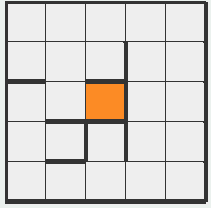
\includegraphics[width=\linewidth]{images/small_mdp}
			\caption{Small}
		\end{subfigure}
		\begin{subfigure}{.45\textwidth}
			\centering
			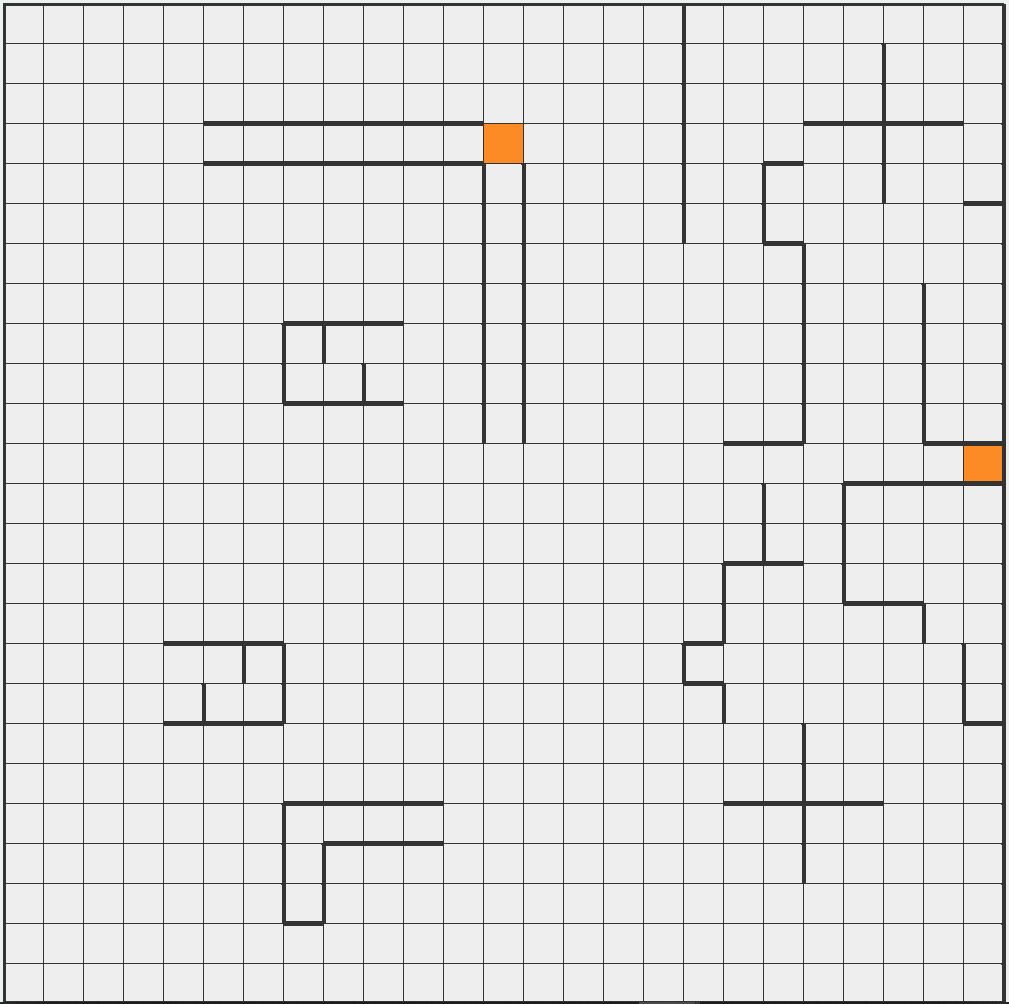
\includegraphics[width=\linewidth]{images/large_mdp}
			\caption{Large}		
		\end{subfigure}
		\caption{Chosen MDPs}
		\label{fig:mdp-viz}%
	\end{figure}%

	\section{Overview of algorithms}
	The three algorithms used to solve the MDPs are described briefly below.
	
	\subsection{Value iteration}
	This is an algorithm that computes the optimal policy by iteratively updating the values (expected utilities) at each state based on the action that maximizes it computed from the transition probabilities, expected utilities and rewards of the neighboring states. The initial values can be initialized arbitrarily. It can be proven that it converges to the optimal values.
	
	\subsection{Policy iteration}
	Value iteration keeps improving the the value function until it converges. However, the optimal policy converges long below the value function. Since the agent only cares about the optimal policy, this is inefficient. Policy iteration works around this problem by iteratively improving the policy at each step and computing the value function according to the new policy instead of repeatedly improving the value function. Policy iteration is also guaranteed to converge to the optimal policy. It often takes fewer iterations to converge than value iteration.
	
	\subsection{Q-learning}
	This is a reinforcement algorithm in which we assume that the transition probabilities and rewards are not known beforehand unlike the previous two algorithms. The agent only knows what are the set of possible states and actions, and can observe the environment current state. In this case, the agent has to actively learn through the experience of interactions with the environment. The Q values are iteratively updated based on the next state that maximizes them. 
	
	An important question is how the agent selects actions during learning. It can either take the action which maximizes the Q value or take other actions which may lead to better rewards. This is known as the exploration-vs-exploitation dilemma. In this assignment, we use the $\epsilon$-greedy policy where at each step the agent takes a random action with some small probability $\epsilon$ instead of taking every action greedily. This encourages exploration. $\epsilon$ can be decreased over time as the agent becomes more confident with its estimate of Q values. This algorithm converges to the optimal policy under certain conditions on learning hyperparameters.
	
	\section{Experiment and analysis}
	The Reinforcement Learning Simulator\footnote{\url{http://www.cs.cmu.edu/~awm/rlsim/}} developed by Rohit Kelkar and Vivek Mehta at Robotics Institute, Carnegie Mellon University was used for experiments. For all three algorithms, the noise probability was set to 0.3 and the threshold for convergence was set to 0.001. For policy iteration, the number of policy evaluations in each iteration was set to 500. For reinforcement learning, different exploration strategies were used by changing the values of $\epsilon$. The learning rate was set to 0.7 initially and decayed according to the formula $1000/(1000 + \text{number of episodes})$. The higher learning rate in the beginning encourages exploration and the lower learning rate towards the end encourages exploitation. The algorithm was run for 10,000 iterations in case of the small MDP and 250,000 iterations for the larger MDP.
	
	For value iteration and policy iteration, the policies and the penalties (negative of the values) are visualized in figures \ref{fig:mdp-viz-small} and \ref{fig:mdp-viz-big}. The shades of blue indicate the penalties. Darker shades mean larger penalties. The number of iterations and the time taken to converge are shown in table \ref{tab:performance}.
	
	\begin{figure}
		\centering
		\begin{subfigure}{.45\textwidth}
			\centering
			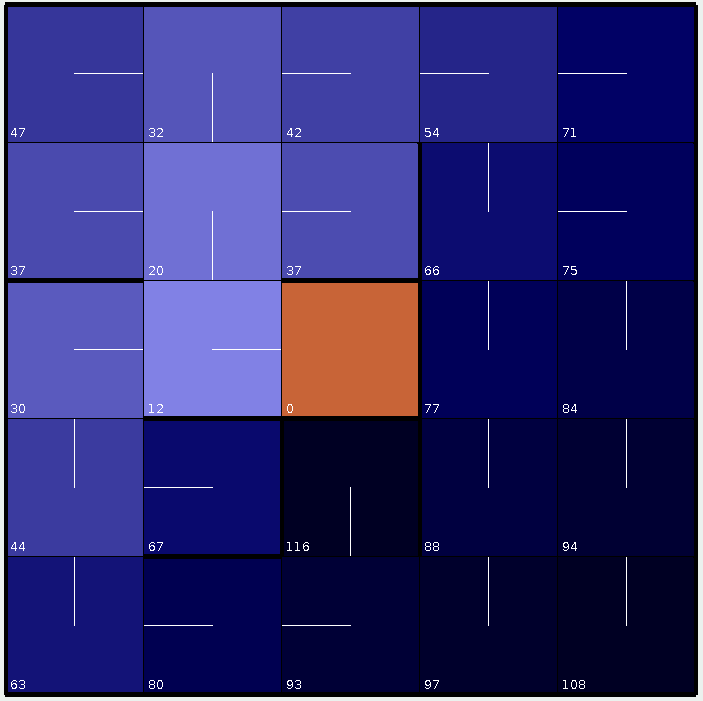
\includegraphics[width=\linewidth]{images/small_vi}
			\caption{Value iteration}
		\end{subfigure}
		\begin{subfigure}{.45\textwidth}
			\centering
			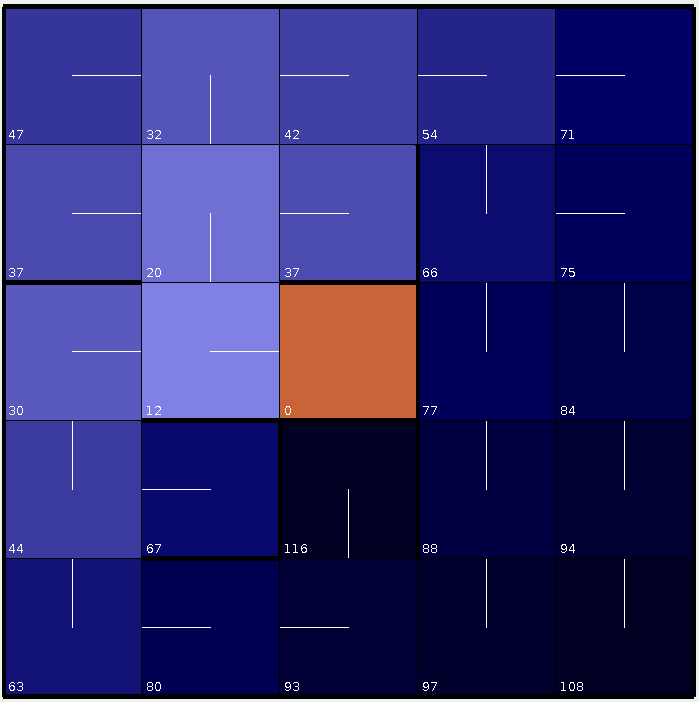
\includegraphics[width=\linewidth]{images/small_pi}
			\caption{Policy iteration}		
		\end{subfigure}
		\caption{Policies and penalties for the small MDP}
		\label{fig:mdp-viz-small}%
	\end{figure}%

\begin{figure}
	\centering
	\begin{subfigure}{.45\textwidth}
		\centering
		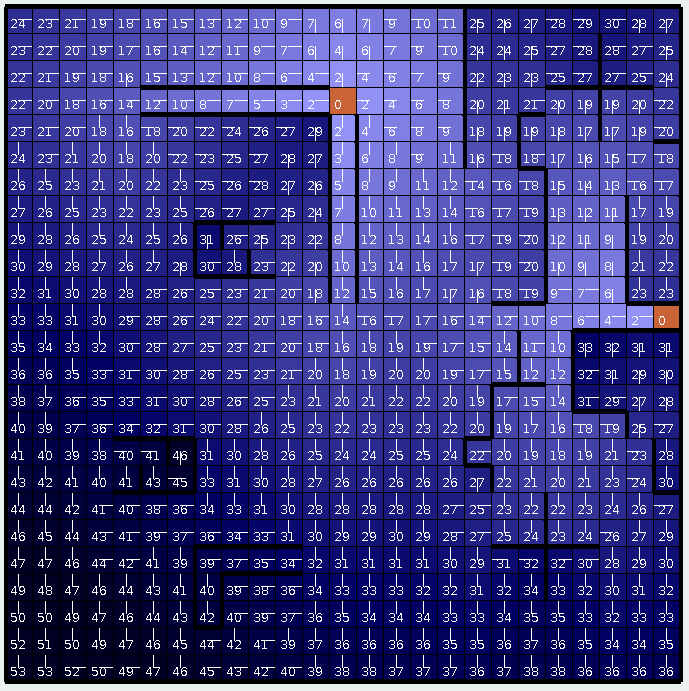
\includegraphics[width=\linewidth]{images/big_vi}
		\caption{Value iteration}
	\end{subfigure}
	\begin{subfigure}{.45\textwidth}
		\centering
		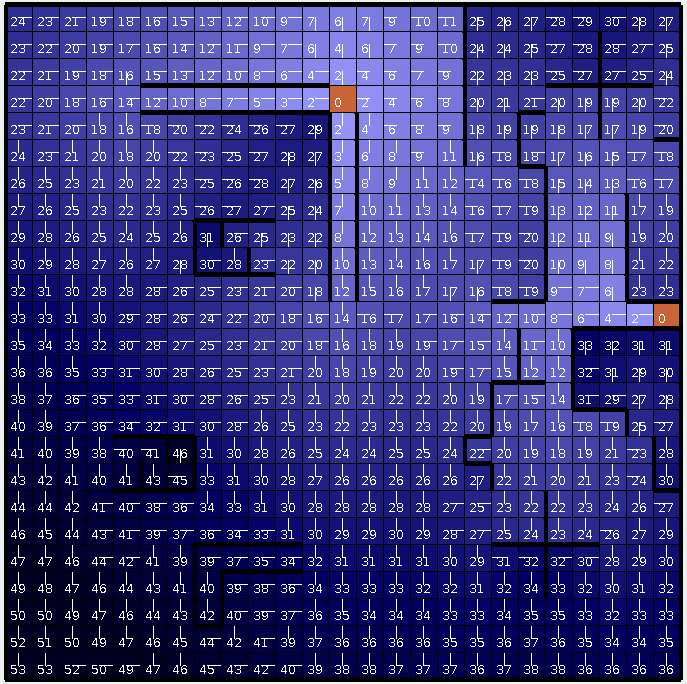
\includegraphics[width=\linewidth]{images/big_pi}
		\caption{Policy iteration}		
	\end{subfigure}
	\caption{Policies and penalties for the large MDP}
	\label{fig:mdp-viz-big}%
\end{figure}%
	
	\begin{table}[!htb]
		\centering
		\captionsetup{justification=centering}
		\caption{Performance of value iteration and policy iteration}
		\label{tab:performance}
		\begin{subtable}{.5\linewidth}
			\centering
			\caption{Small MDP}
			\begin{tabular}{ccc}
				\toprule
				 & \textbf{VI} & \textbf{PI} \\
				 \midrule
				 Iterations & 50 & 6 \\
				 \midrule
				 Time (ms) & 13 & 6 \\
				 \bottomrule
			\end{tabular}
		\end{subtable}%
		\begin{subtable}{.5\linewidth}
			\centering
			\caption{Large MDP}
			\begin{tabular}{ccc}
				\toprule
				& \textbf{VI} & \textbf{PI} \\
				\midrule
				Iterations & 91 & 8 \\
				\midrule
				Time (ms) & 340 & 866 \\
				\bottomrule
			\end{tabular}
		\end{subtable} 
	\end{table}

	We can observe that both value iteration and policy iteration found the same policy in both problems. This is expected as both value iteration and policy iteration provably find the optimal policy. For the small MDP, policy iteration is faster than value iteration in terms of both time and the number of iterations needed to converge. However, for the large MDP, policy iteration needs fewer iterations than value iteration but runs for a longer time. To understand how problem size affects running time of the two algorithms, we look at their computational complexity. The efficiencies of value iteration and policy iteration are $O(S^2 A)$ and $O(S^2 N)$ respectively. Here, $S$ is the number of states in the problem, $A$ is the number of possible actions at each state and $N$ is the number of policy evaluations in each policy iteration. Even though policy iteration takes fewer iterations than value iteration, each iteration is more expensive. This especially becomes a problem for large state spaces since even a small increase in the number of iterations taken by policy iteration will result in a large increase in time required to converge. As both of them are optimal, we can conclude that value iteration should be used for small MDPs and policy iteration for large MDPs.
	
	The policies and values at different iterations for the two algorithms are shown in figures \ref{fig:mdp-vi-iter-small}, \ref{fig:mdp-pi-iter-small}, \ref{fig:mdp-vi-iter-large} and \ref{fig:mdp-pi-iter-large}. We can observe how they slowly improve and converge to their optima. In the case of value iteration, the policy converges before the values. For the small MDP, the policy converges as early as the 20th iteration. This shows that value iteration is inefficient for small MDPs.
	
	\begin{figure}
		\centering
		\begin{subfigure}[t]{.18\textwidth}
			\centering
			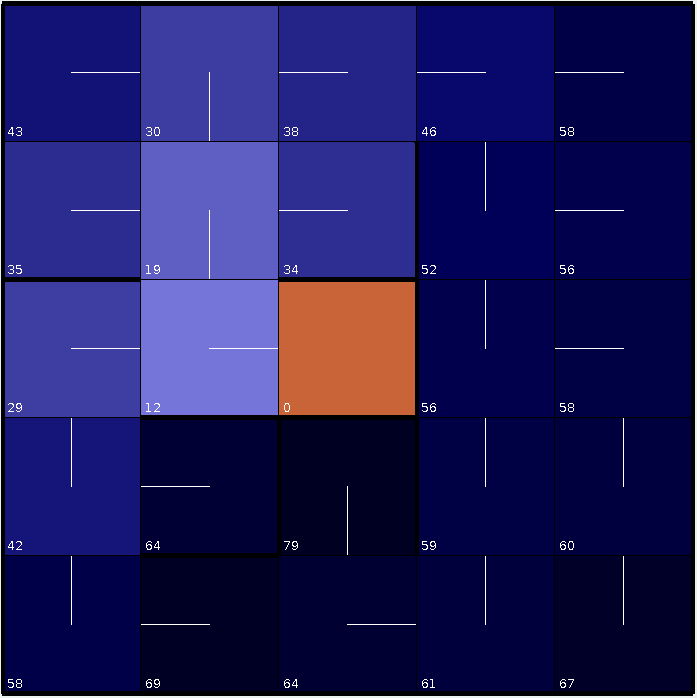
\includegraphics[width=\linewidth]{images/small_vi_10}
			\caption{Iteration 10}
		\end{subfigure}
		\begin{subfigure}[t]{.18\textwidth}
			\centering
			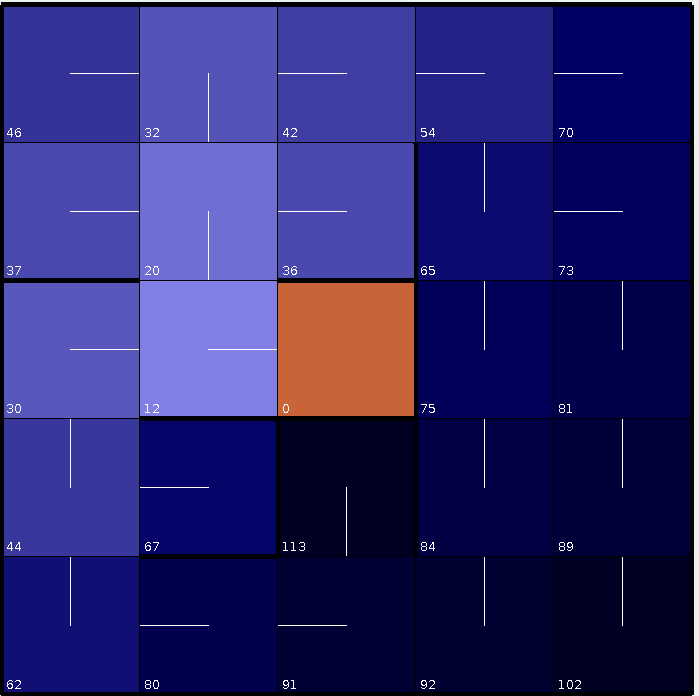
\includegraphics[width=\linewidth]{images/small_vi_20}
			\caption{Iteration 20}
		\end{subfigure}
		\begin{subfigure}[t]{.18\textwidth}
			\centering
			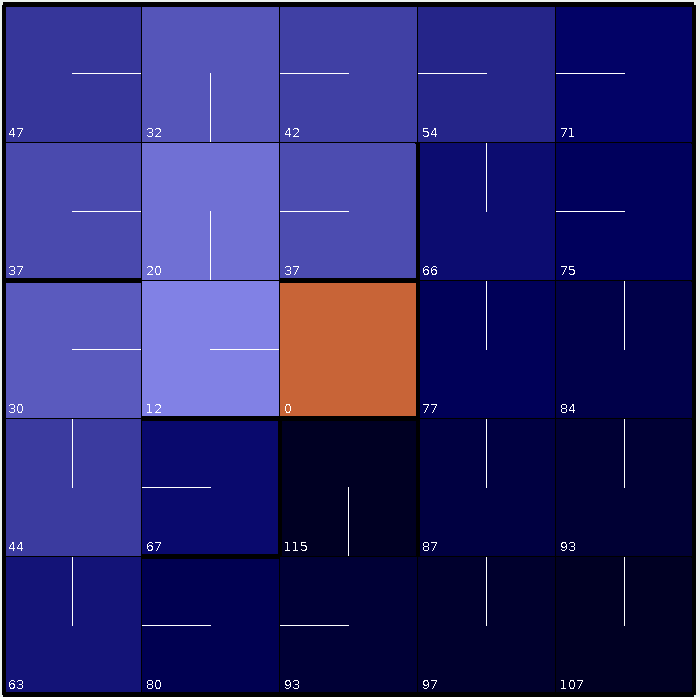
\includegraphics[width=\linewidth]{images/small_vi_30}
			\caption{Iteration 30}
		\end{subfigure}
		\begin{subfigure}[t]{.18\textwidth}
			\centering
			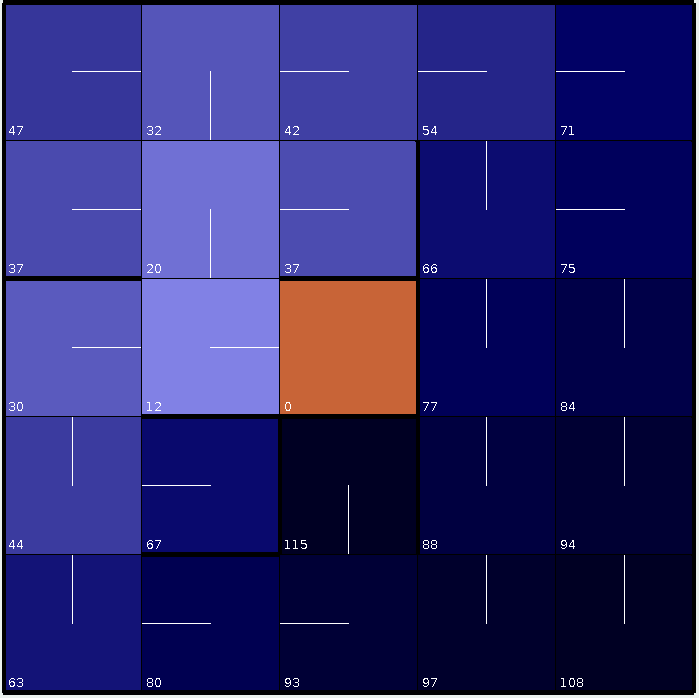
\includegraphics[width=\linewidth]{images/small_vi_40}
			\caption{Iteration 40}
		\end{subfigure}
		\begin{subfigure}[t]{.18\textwidth}
			\centering
			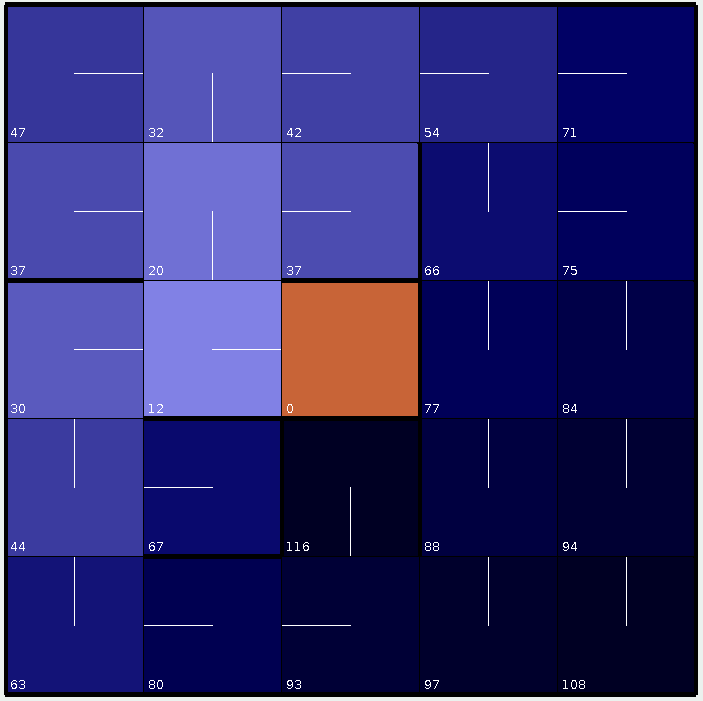
\includegraphics[width=\linewidth]{images/small_vi}
			\caption{Iteration 50 (convergence)}
		\end{subfigure}
		\caption{Value iteration: policies and values after different iterations for small MDP}
		\label{fig:mdp-vi-iter-small}%
	\end{figure}%

	\begin{figure}
		\centering
		\begin{subfigure}{.3\textwidth}
			\centering
			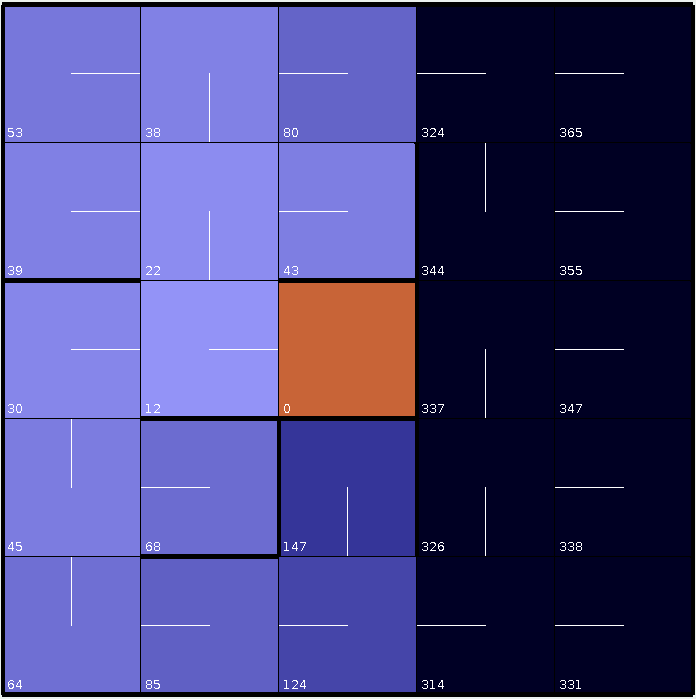
\includegraphics[width=\linewidth]{images/small_pi_2}
			\caption{Iteration 2}
		\end{subfigure}
		\begin{subfigure}{.3\textwidth}
			\centering
			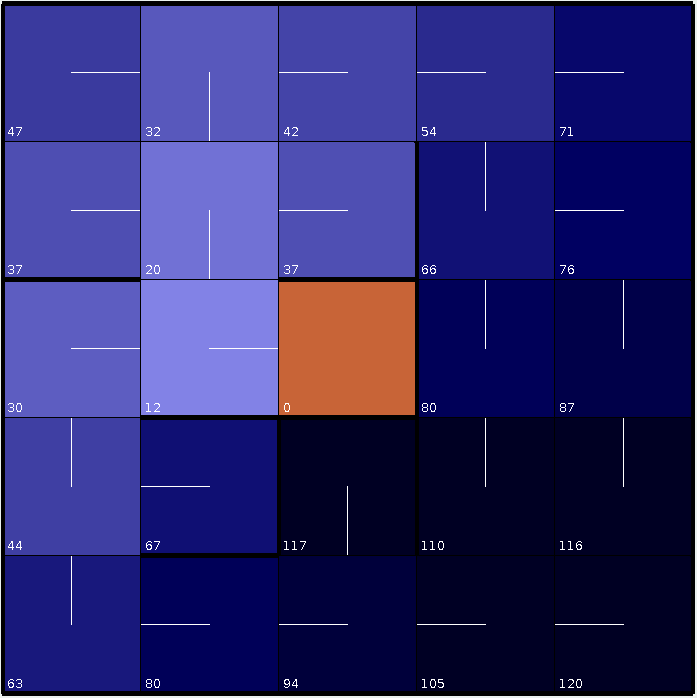
\includegraphics[width=\linewidth]{images/small_pi_4}
			\caption{Iteration 4}
		\end{subfigure}
		\begin{subfigure}{.3\textwidth}
			\centering
			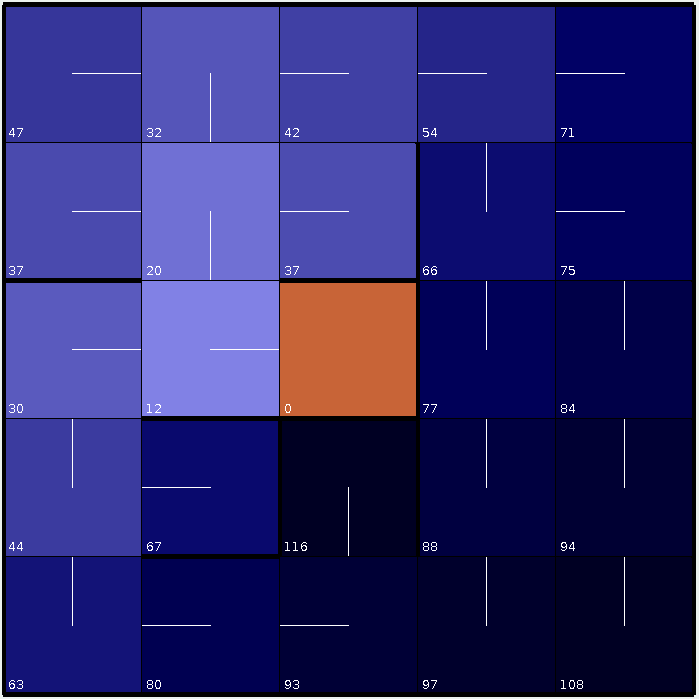
\includegraphics[width=\linewidth]{images/small_pi_6}
			\caption{Iteration 6 (convergence)}
		\end{subfigure}
		\caption{Policy iteration: policies and values after different iterations for small MDP}
		\label{fig:mdp-pi-iter-small}%
	\end{figure}%

	\begin{figure}
		\centering
		\begin{subfigure}{.3\textwidth}
			\centering
			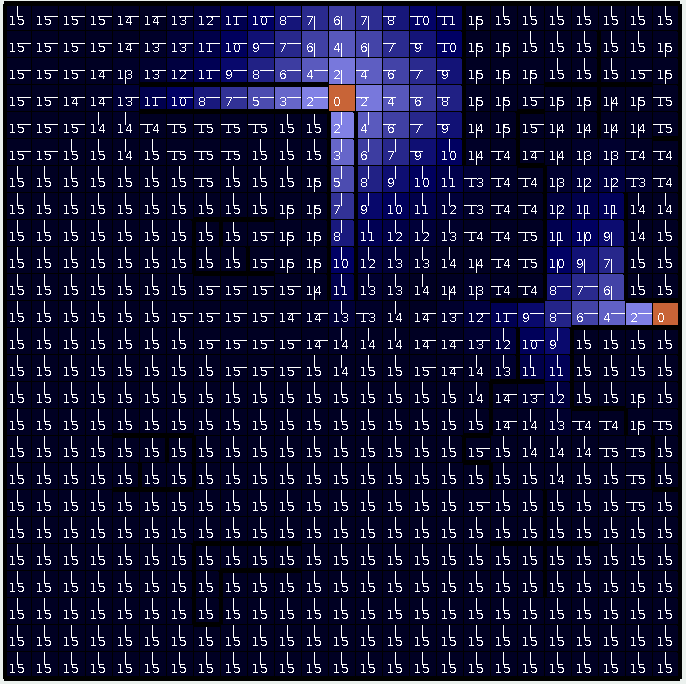
\includegraphics[width=\linewidth]{images/big_vi_15}
			\caption{Iteration 15}
		\end{subfigure}
		\begin{subfigure}{.3\textwidth}
			\centering
			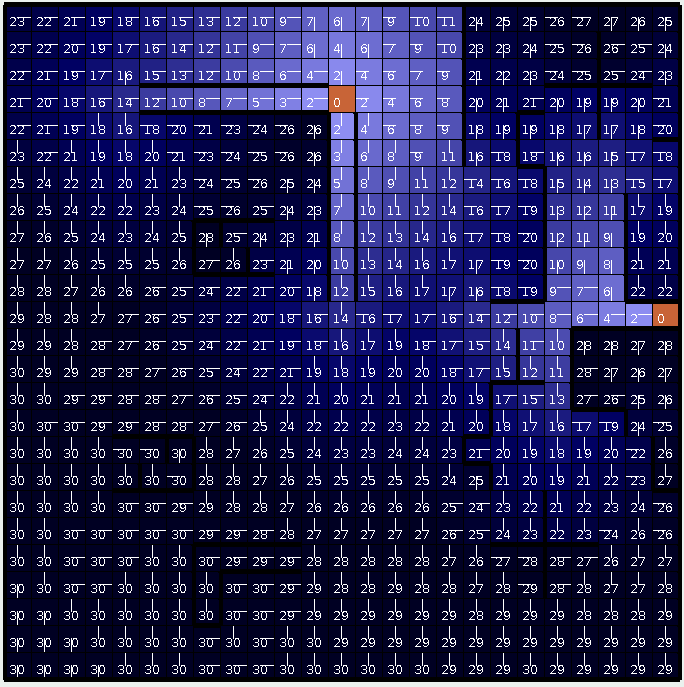
\includegraphics[width=\linewidth]{images/big_vi_30}
			\caption{Iteration 30}
		\end{subfigure}
		\begin{subfigure}{.3\textwidth}
			\centering
			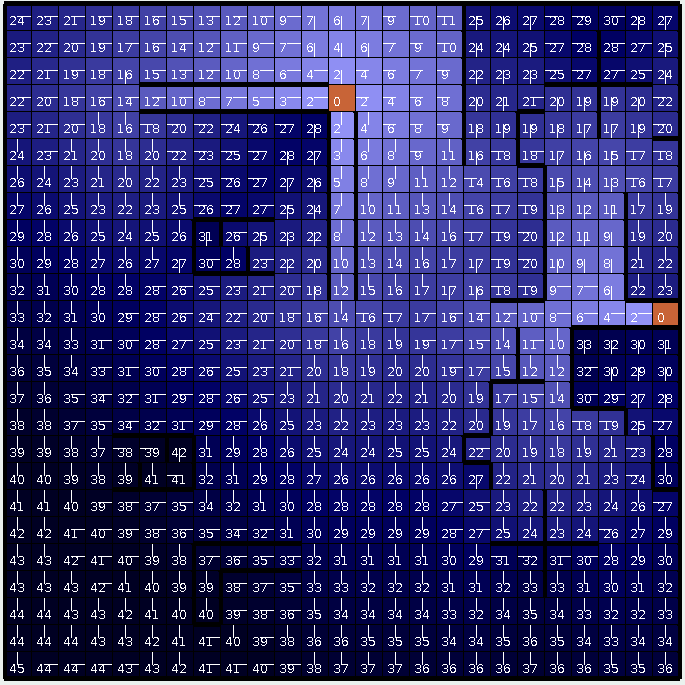
\includegraphics[width=\linewidth]{images/big_vi_45}
			\caption{Iteration 45}
		\end{subfigure}
		\begin{subfigure}{.3\textwidth}
			\centering
			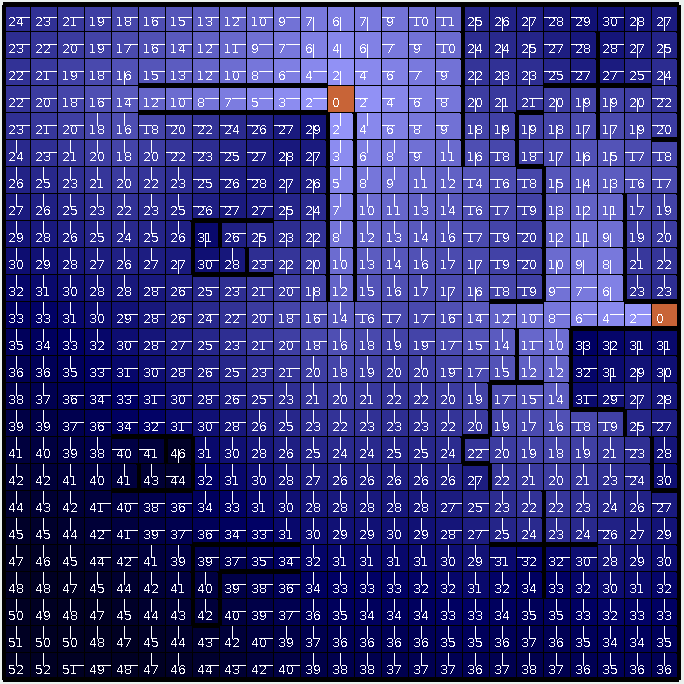
\includegraphics[width=\linewidth]{images/big_vi_60}
			\caption{Iteration 60}
		\end{subfigure}
		\begin{subfigure}{.3\textwidth}
			\centering
			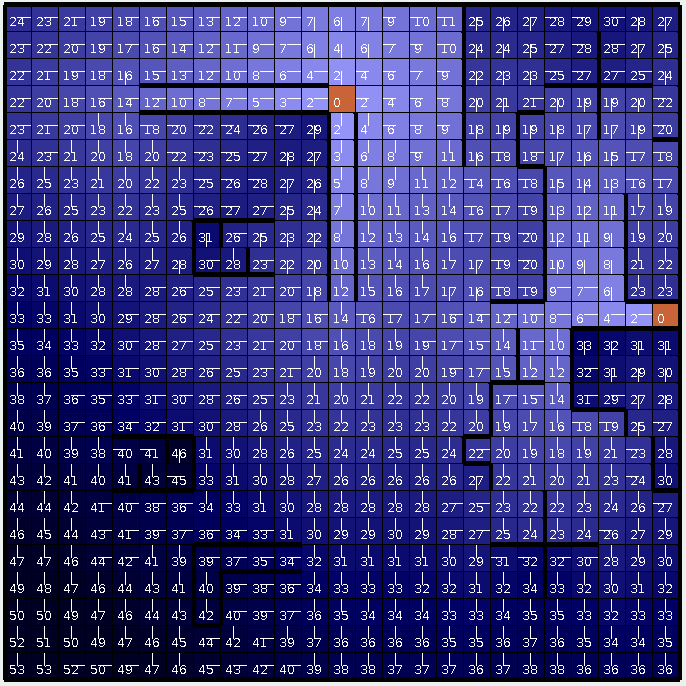
\includegraphics[width=\linewidth]{images/big_vi_75}
			\caption{Iteration 75}
		\end{subfigure}
		\begin{subfigure}{.3\textwidth}
			\centering
			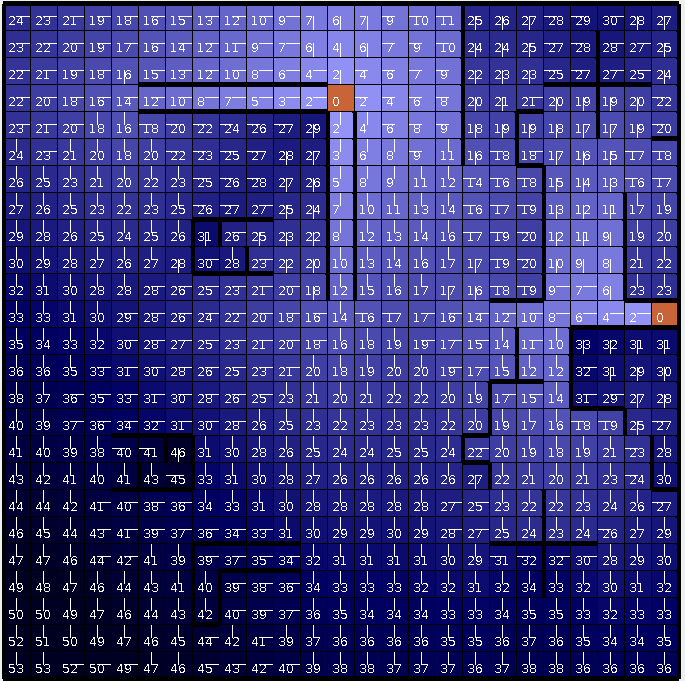
\includegraphics[width=\linewidth]{images/big_vi_91}
			\caption{Iteration 91 (convergence)}
		\end{subfigure}
		\caption{Value iteration: policies and values after different iterations for large MDP}
		\label{fig:mdp-vi-iter-large}%
	\end{figure}%

	\begin{figure}
		\centering
		\begin{subfigure}[t]{.23\textwidth}
			\centering
			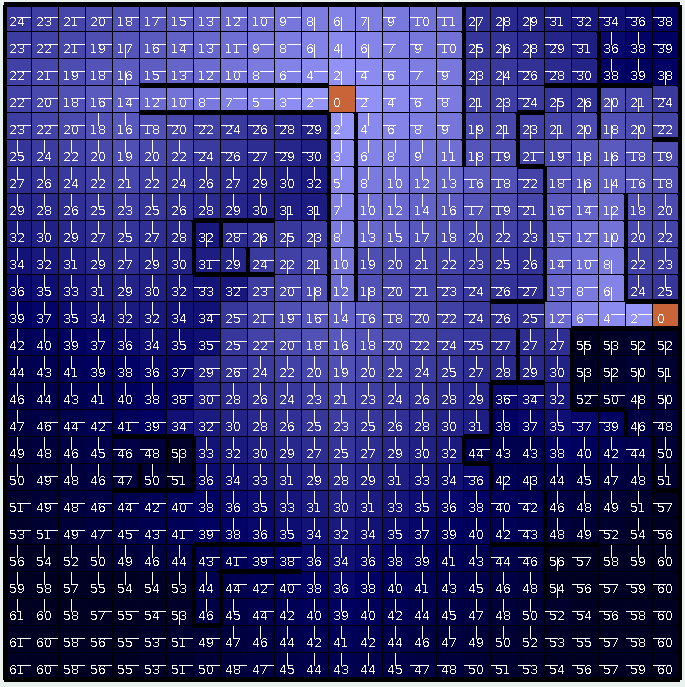
\includegraphics[width=\linewidth]{images/big_pi_2}
			\caption{Iteration 2}
		\end{subfigure}
		\begin{subfigure}[t]{.23\textwidth}
			\centering
			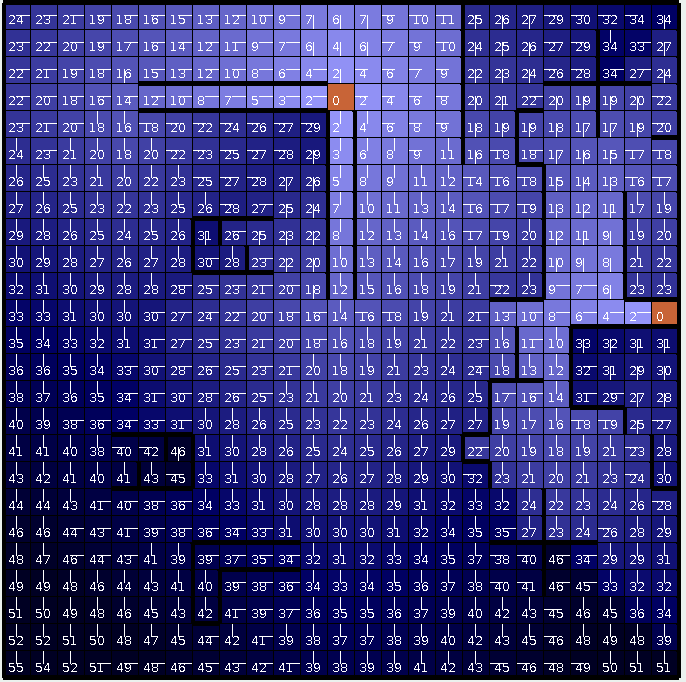
\includegraphics[width=\linewidth]{images/big_pi_4}
			\caption{Iteration 4}
		\end{subfigure}
		\begin{subfigure}[t]{.23\textwidth}
			\centering
			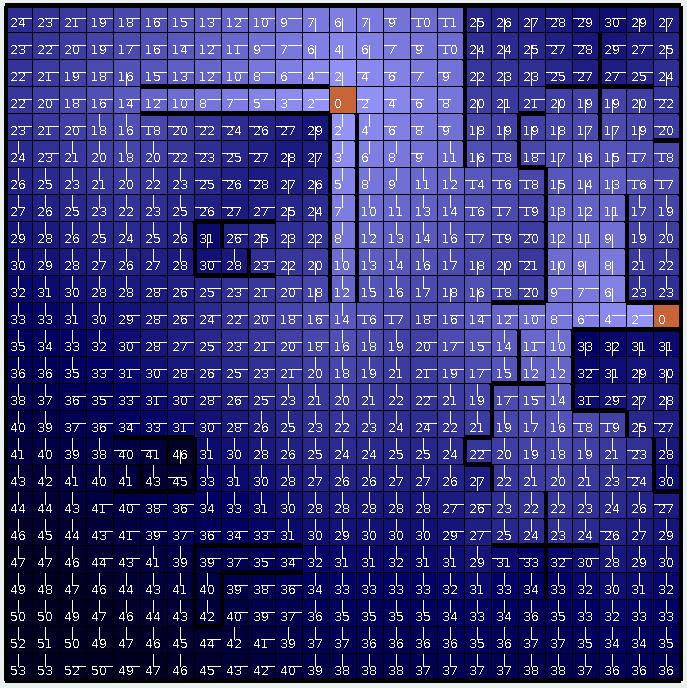
\includegraphics[width=\linewidth]{images/big_pi_6}
			\caption{Iteration 6}
		\end{subfigure}
		\begin{subfigure}[t]{.23\textwidth}
			\centering
			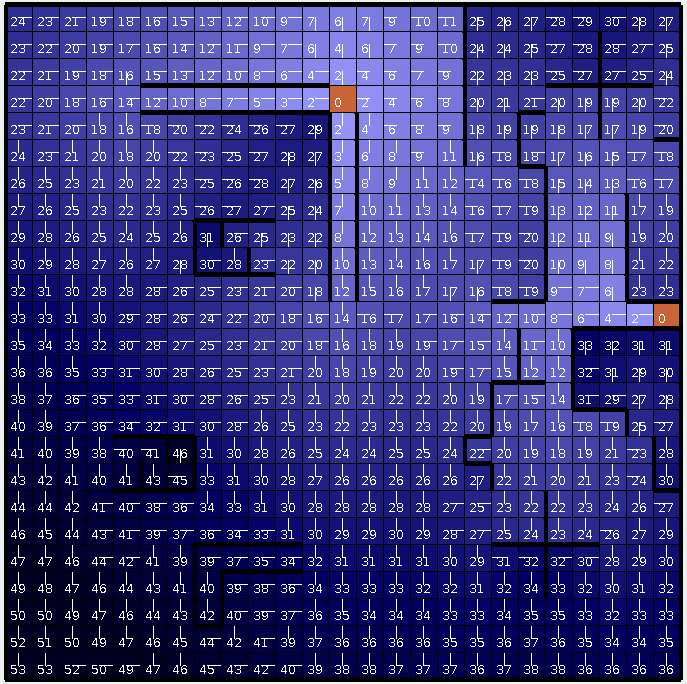
\includegraphics[width=\linewidth]{images/big_pi}
			\caption{Iteration 8 (convergence)}
		\end{subfigure}
		\caption{Policy iteration: policies and values after different iterations for large MDP}
		\label{fig:mdp-pi-iter-large}%
	\end{figure}%
	
	For Q-learning, the policies and Q values for different values of $\epsilon$ are shown in figures \ref{fig:mdp-ql-small} and \ref{fig:mdp-ql-large}. For the small MDP, we can observe that it hasn't converged to the optimal policy in any case. For the first four cases, it gets 3--6 states wrong. The best performance is obtained with $\epsilon = 0.5$, the highest $\epsilon$ tried, where it gets only one state wrong. This shows the importance of exploration in Q-learning. If the exploration is too low, Q-learning may not converge to the optimal policy. Even for the large MDP, Q-learning could not find the optimal policy for any $\epsilon$. All exploration strategies resulted in some portions of the grid being mapped out correctly. However, states near walls, tunnels and traps noticeably have incorrect policies. For large values of $\epsilon$, the policies look better overall, again emphasizing the importance of exploration. Even though Q-learning did not result in optimal policies, it is nevertheless remarkable to observe how it gets most of the decisions right inspite of not having knowledge of the environment and without modeling transition probabilities and rewards.
	
	\begin{figure}
		\centering
		\begin{subfigure}{.3\textwidth}
			\centering
			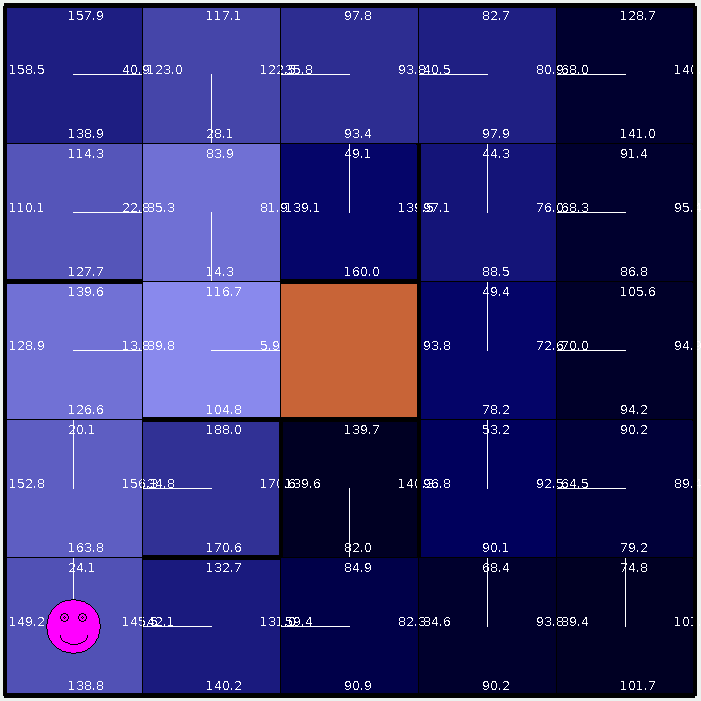
\includegraphics[width=\linewidth]{images/small_ql_0}
			\caption{$\epsilon = 0$}
		\end{subfigure}
		\begin{subfigure}{.3\textwidth}
			\centering
			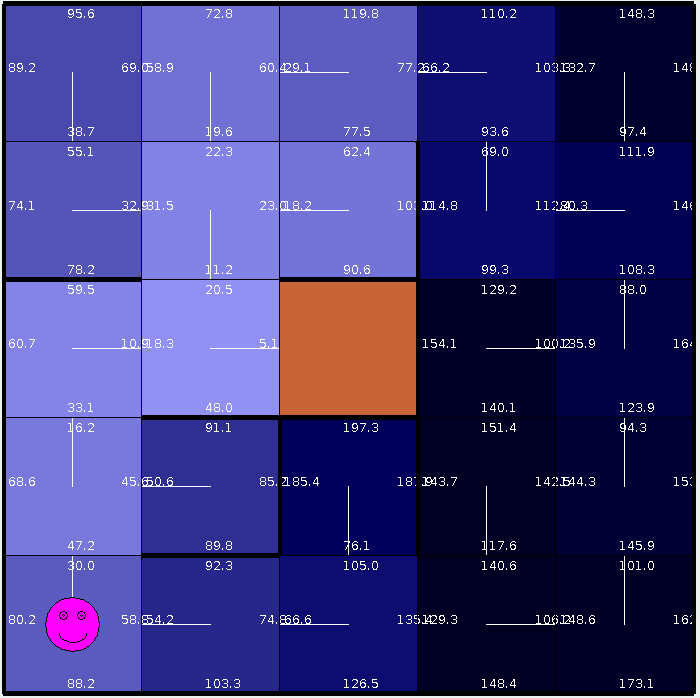
\includegraphics[width=\linewidth]{images/small_ql_01}
			\caption{$\epsilon = 0.1$}
		\end{subfigure}
		\begin{subfigure}{.3\textwidth}
			\centering
			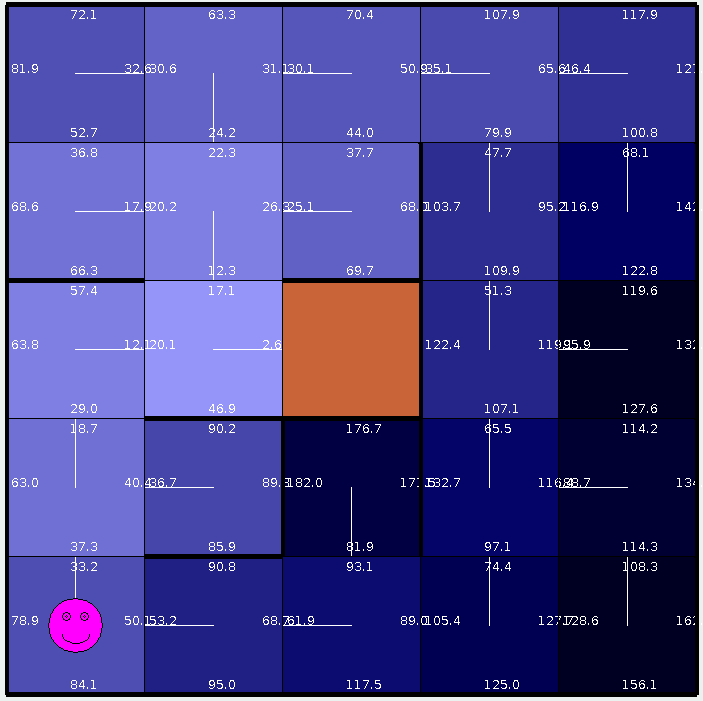
\includegraphics[width=\linewidth]{images/small_ql_02}
			\caption{$\epsilon = 0.2$}
		\end{subfigure}
		\begin{subfigure}{.3\textwidth}
			\centering
			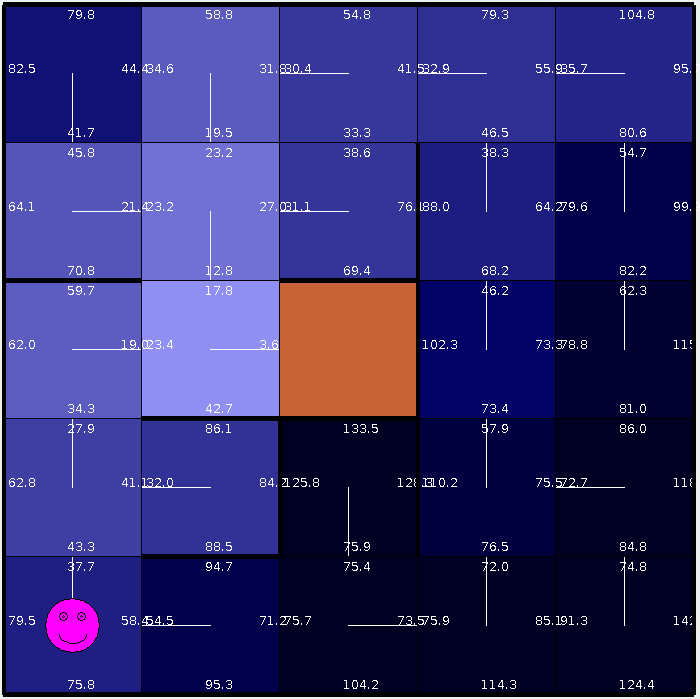
\includegraphics[width=\linewidth]{images/small_ql_03}
			\caption{$\epsilon = 0.3$}		
		\end{subfigure}
		\begin{subfigure}{.3\textwidth}
			\centering
			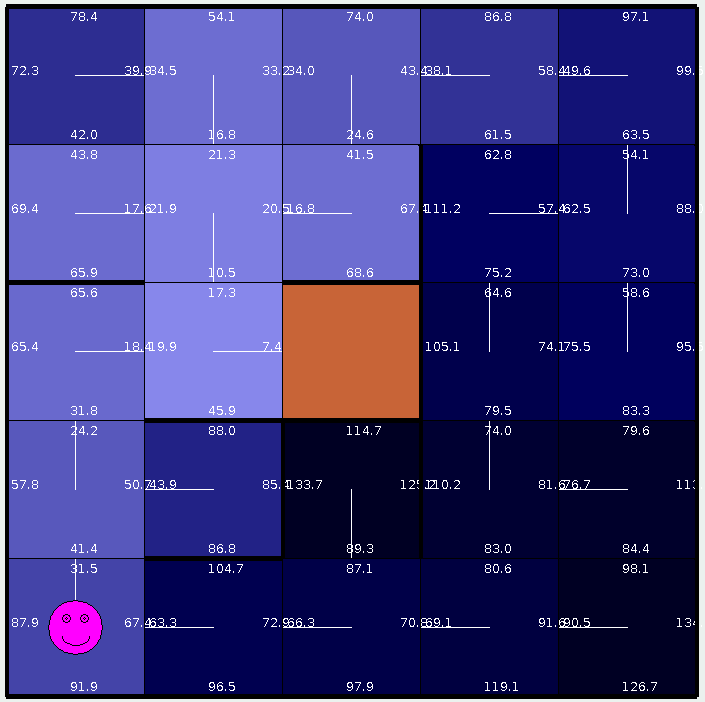
\includegraphics[width=\linewidth]{images/small_ql_04}
			\caption{$\epsilon = 0.4$}		
		\end{subfigure}
		\begin{subfigure}{.3\textwidth}
			\centering
			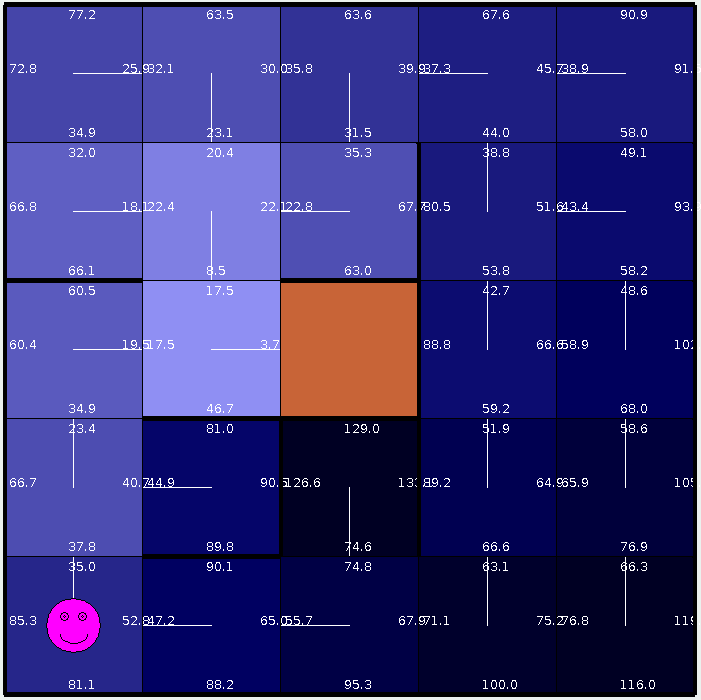
\includegraphics[width=\linewidth]{images/small_ql_05}
			\caption{$\epsilon = 0.5$}		
		\end{subfigure}
		\caption{Q-learning: policies and Q values for small MDP}
		\label{fig:mdp-ql-small}%
	\end{figure}%

	\begin{figure}
		\centering
		\begin{subfigure}{.3\textwidth}
			\centering
			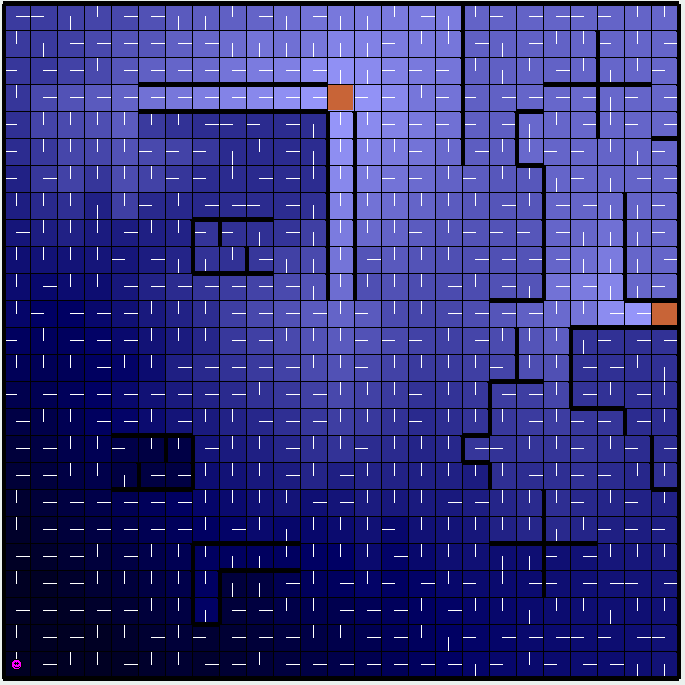
\includegraphics[width=\linewidth]{images/big_ql_0}
			\caption{$\epsilon = 0$}
		\end{subfigure}
		\begin{subfigure}{.3\textwidth}
			\centering
			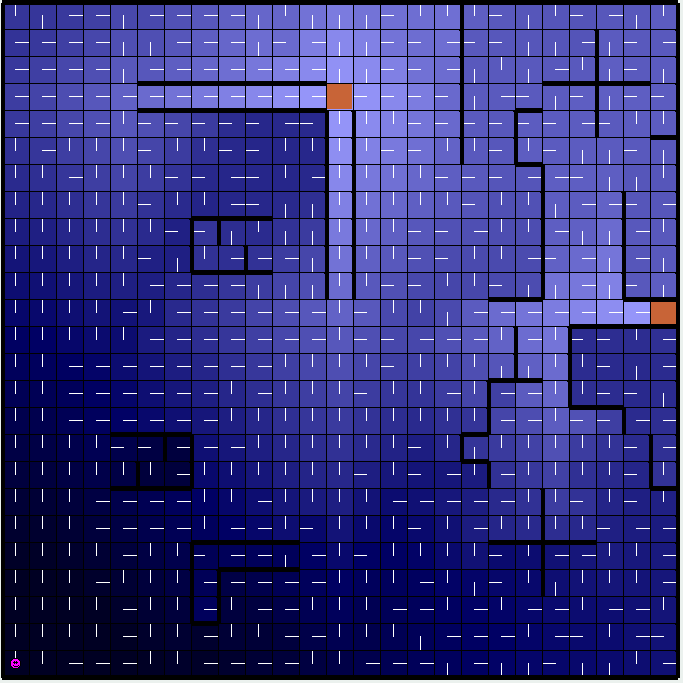
\includegraphics[width=\linewidth]{images/big_ql_01}
			\caption{$\epsilon = 0.1$}
		\end{subfigure}
		\begin{subfigure}{.3\textwidth}
			\centering
			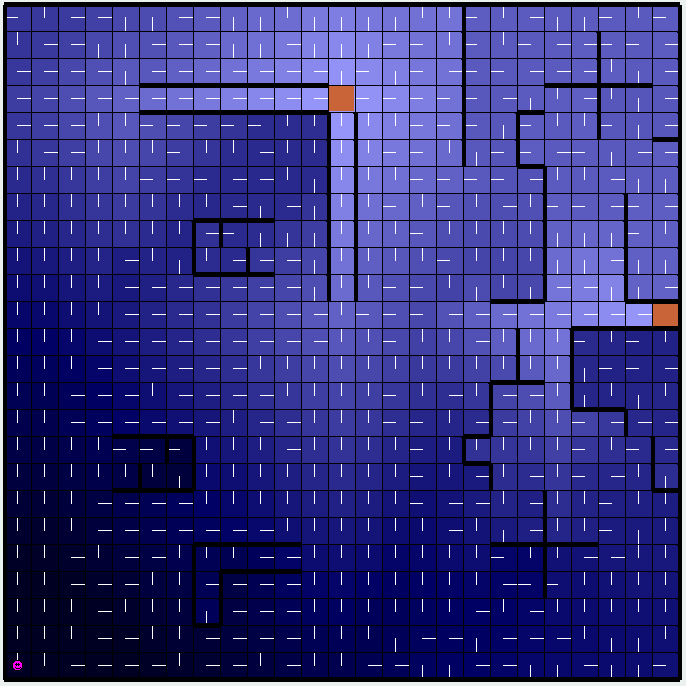
\includegraphics[width=\linewidth]{images/big_ql_02}
			\caption{$\epsilon = 0.2$}
		\end{subfigure}
		\begin{subfigure}{.3\textwidth}
			\centering
			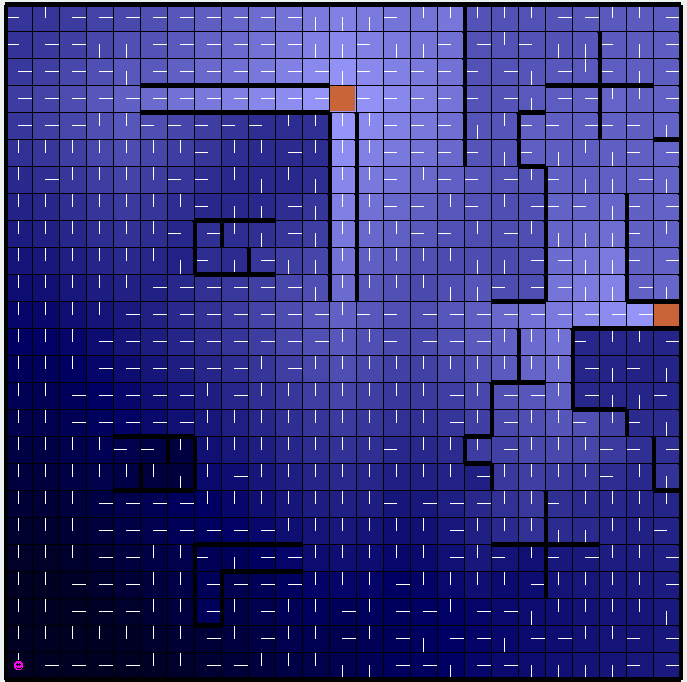
\includegraphics[width=\linewidth]{images/big_ql_03}
			\caption{$\epsilon = 0.3$}		
		\end{subfigure}
		\begin{subfigure}{.3\textwidth}
			\centering
			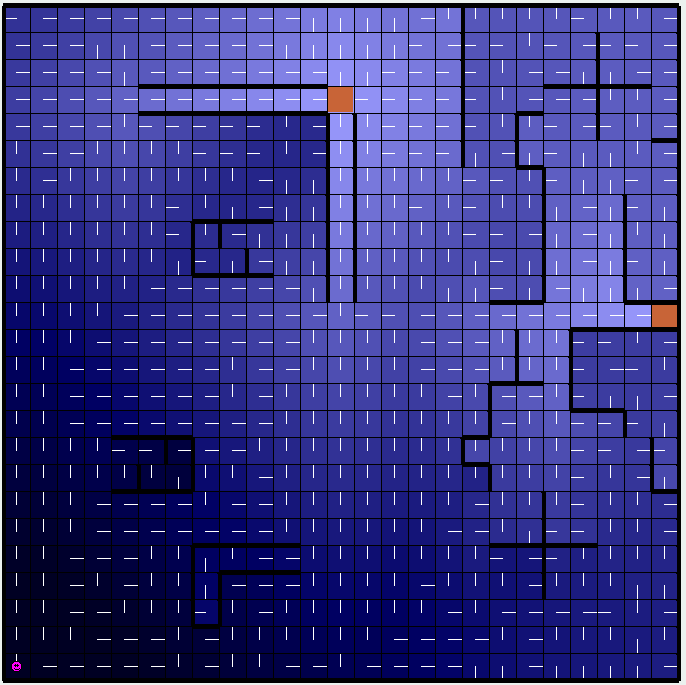
\includegraphics[width=\linewidth]{images/big_ql_04}
			\caption{$\epsilon = 0.4$}		
		\end{subfigure}
		\begin{subfigure}{.3\textwidth}
			\centering
			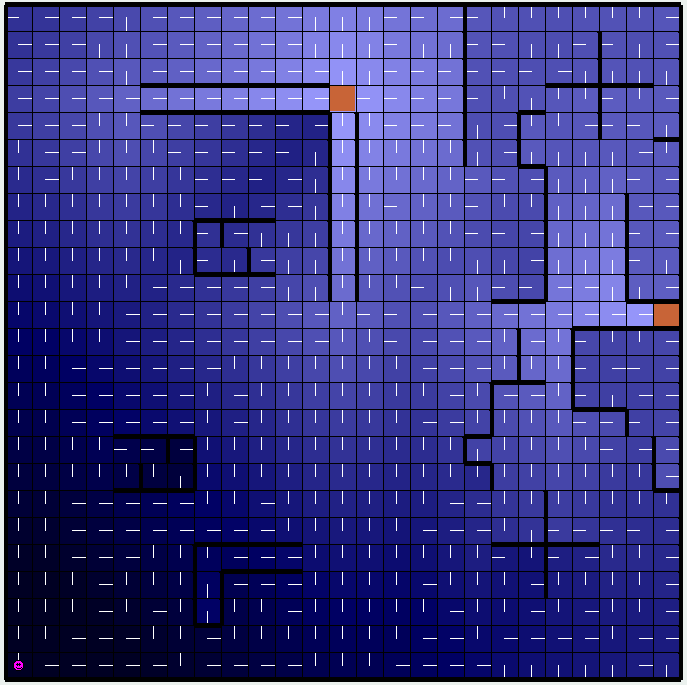
\includegraphics[width=\linewidth]{images/big_ql_05}
			\caption{$\epsilon = 0.5$}		
		\end{subfigure}
		\caption{Q-learning: policies for large MDP}
		\label{fig:mdp-ql-large}%
	\end{figure}%
	
\end{document}